\section{Grundlagen}
\subsection{Melodie}
\subsection{Harmonie}
\subsection{Rhytmus}

\subsection{Tonleitern}
Eine Tonleiter oder Ton-Skala ist in der Musik eine Reihe von der Tonhöhe nach geordneten Tönen, 
jenseits derer die Tonreihe in der Regel wiederholbar ist. In den meisten Fällen hat eine Tonleiter 
den Umfang einer Oktave. Weit verbreitet sind diatonische Tonleitern in Dur und Moll oder die 
Kirchentonleitern. Tonleitern sind durch Tonabstände definiert.

\begin{figure}[htbp]
    \centering
    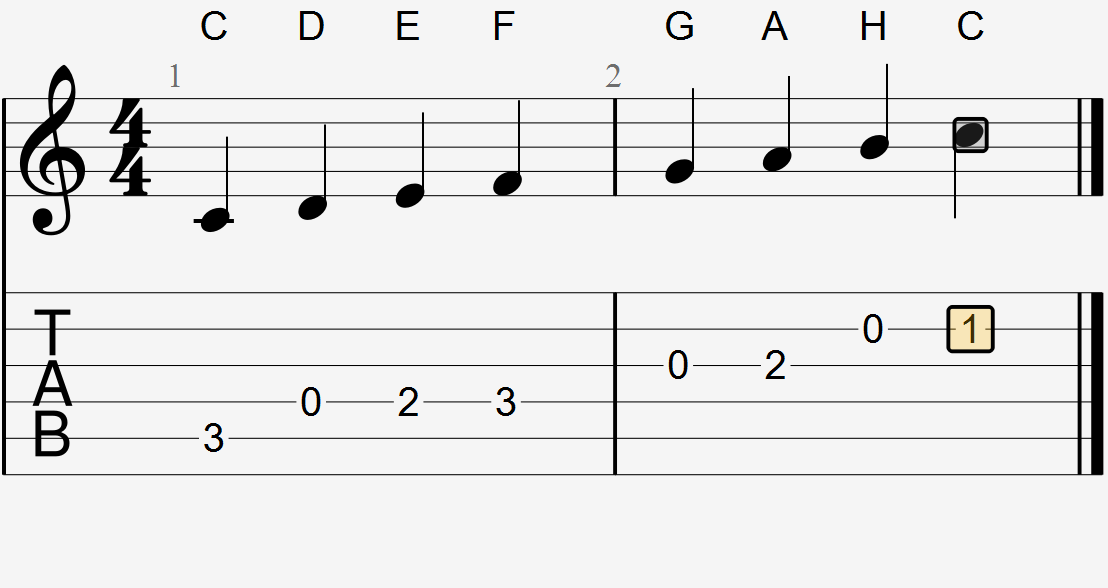
\includegraphics[width=0.8\textwidth]{images/C_Dur_Tonika}
\end{figure}

\subsection{Akkorde}
\subsection{Tonarten}
\subsubsection{Szenariobasiertes Testen}

